%  astrochem.tex - Astrochem documentation manual
%
%  Copyright (c) 2006-2010 Sebastien Maret
%
%  This file is part of Astrochem.
%
%  Astrochem is free software: you can redistribute it and/or modify
%  it under the terms of the GNU General Public License as published
%  by the Free Software Foundation, either version 3 of the License,
%  or (at your option) any later version.
%
%  Astrochem is distributed in the hope that it will be useful, but
%  WITHOUT ANY WARRANTY; without even the implied warranty of
%  MERCHANTABILITY or FITNESS FOR A PARTICULAR PURPOSE.  See the GNU
%  General Public License for more details.
%
%  You should have received a copy of the GNU General Public License
%  along with Astrochem.  If not, see <http://www.gnu.org/licenses/>.

\documentclass[a4paper,12pt]{article}

\usepackage{url,graphicx,fancyvrb,html}
\usepackage[hmargin=2.2cm,vmargin=2.5cm]{geometry}
\usepackage{verbatim} 
\usepackage{natbib}

\newcommand{\aap}{A\&A}
\newcommand{\apj}{ApJ}
\newcommand{\mnras}{MNRAS}

% FixMe: Replace the following values with a Makefile
\newcommand{\version}{0.1}
\newcommand{\updated}{November 5th, 2010}
\newcommand{\bugreport}{\url{sebastien.maret@obs.ujf-grenoble.fr}}

\newcommand{\conc}[1]{n(\mathrm{#1})}

\begin{document}

\VerbatimFootnotes

\thispagestyle{empty}
\vspace*{5cm}

\noindent
\huge{\textbf{Astrochem}}

\begin{latexonly}
  \vskip4pt \hrule height 4pt width \hsize
\end{latexonly}

\begin{flushright}
  \noindent
  \small{
    Documentation Manual\\
    For Astrochem version \version\\
    \updated
  }
\end{flushright}

\noindent
\large{\textbf{S\'ebastien Maret}\\
\small{Laboratoire d'Astrophysique de Grenoble\\}

\noindent
\large{\textbf{Edwin A. Bergin}}\\
\small{University of Michigan}\\

\newpage
\vspace*{20cm}

\small{
  \noindent This manual documents Astrochem, a code to compute the
  abundance of chemical species in the interstellar medium. It
  corresponds to Astrochem version \version.
  Please report any errors in this manual to \bugreport.
  \\ \\ \noindent Copyright \copyright \, 2006-2010 S\'ebastien
  Maret
}

\section{What is Astrochem?}
\label{sec:what-astrochem}

Astrochem is a code to compute the abundances of chemical species in
the interstellar medium, as function of time. It is designed to study
the chemistry in a variety of astronomical objects, including diffuse
clouds, dense clouds, photodissociation regions, prestellar cores,
protostars, and protostellar disks. Astrochem reads a network of
chemical reactions from a text file, builds up a system of kinetic
rates equations, and solve it using a state-of-the-art stiff ordinary
differential equation (ODE) solver. The Jacobian matrix of the system
is computed implicitly, so the resolution of the system is extremely
fast: large networks containing several thousands of reactions are
usually solved in a few seconds. A variety of gas phase process are
considered, as well as simple gas-grain interactions, such as the
freeze-out and the desorption via several mechanisms (thermal
desorption, cosmic-ray desorption and photo-desorption). The computed
abundances are written in text files, and can be plotted in different
ways with the tools provided with Astrochem. Chemical reactions and
their rates are written in a format which is meant to be easy to read
and to edit. A tool to convert the chemical networks from standard
databases (OSU, UMIST) into this format is provided. Astrochem is
written in C, and its source code is distributed under the terms of
the GNU General Public License (GPL).

\section{The model}
\label{sec:model}

To understand what Astrochem does, maybe the easiest is to take a
simple example. Let us assume that we want to compute the
abundance of HCO$^{+}$ as a function of time. For a sake of
simplicity, we assumed that it is formed solely through the reaction:

\begin{equation}
  \mathrm{H_{3}^{+} + CO \rightarrow HCO^{+} + H_{2}}
\end{equation}

\noindent
with a rate $k_{1}$. Furthermore, we assume that it is destroyed by
the following reaction:

\begin{equation}
  \mathrm{HCO^{+} + e^{-} \rightarrow H + CO}
\end{equation}

\noindent
with a rate constant $k_{2}$. The derivative of the HCO$^{+}$
concentration (i.e. the number of HCO$^{+}$ per volume unit), that we
note $\conc{HCO^{+}}$ is given by the following kinetic equation:

\begin{equation}
  \frac{d\conc{HCO^{+}}}{dt} = k_{1} \conc{H_{3}^{+}} \conc{CO}
  - k_{2} \conc{HCO^{+}} \conc{e^{-}}
\end{equation}

\noindent
Here the first part of the left-hand of the equation correspond to a
formation rate, and the second part to a destruction rate.

More generaly, we can write the time derivative of the concentration
of a species $x_{i}$ as:

\begin{equation}
  \frac{d\conc{x_{i}}}{dt} = \sum_j k_{j} \prod_l \conc{x_{l}}
    - \sum_m k_{m} \prod_o \conc{x_{o}}
\end{equation}

\noindent
where the $j$ summation index goes over all $x_{i}$ formation
reaction, and the $l$ product index goes each reactant of that
reaction (e.g. 2 for a two-body reaction). Similarly, the $m$ index
goes over each destruction reaction, and the $o$ index goes over each
reactant of that reaction.

In order to determine the concentration of each species as a function
of time, one need to solve the system of $n_\mathrm{s}$ equations for
a set of initial conditions, with $n_\mathrm{s}$ the number of species
in the chemical network. These are ordinary differential equation
(ODE), that may be solved by different methods (Euler method,
Runge-Kutta method, etc.). One difficulty is that the ODE system is
usually \emph{stiff}, because of the different timescales considered
in the code; for example, a neutral-neutral reaction is typically
several orders of magnitude slower than a ion-neutral
reaction. Another characteristic of the system is that it is
\emph{sparse}; many species do not react together, resulting in a
large number of zeros in the Jacobian matrix of the
system\footnote{The Jacobian matrix is a $n_\mathrm{s}^2$ elements
  square matrix, whose elements are defined as
  \begin{equation}
    J_{i,j} = \frac{\partial
      \dot\conc{x_{i}}}{\partial \conc{x_{i}}}
  \end{equation}
  \noindent
  with:
  \begin{equation}
    \dot\conc{x_{i}} = \frac{d \conc{x_{i}}}{dt}
  \end{equation}}.
  
\subsection{Gas-phase reactions}
\label{sec:gas-phase-reactions}

\begin{equation}
  k = \alpha  \left( \frac{T}{300} \right)^\beta  \mathrm{exp} \left(
    -\frac{\gamma}{T} \right)
  \label{eq:arrhenius}
\end{equation}

\subsubsection{Cosmic-ray ionization}
\label{sec:cosm-ray-ioniz}

\begin{equation}
  k = \alpha  \zeta
  \label{eq:cosmic-ray-ionization}
\end{equation}

\subsubsection{Photo-ionization and photo-dissociation}
\label{sec:photo-ioniz-photo}

\begin{equation}
  k = \alpha \mathrm{exp} \left( -\gamma A_{v} \right) \chi
  \label{eq:photo-ionization}
\end{equation}

\subsection{Gas-grain interactions}
\label{sec:gas-grain-inter}

\subsubsection{Electron attachment and ion neutralization on grains}
\label{sec:electr-attachm-ion}

\begin{equation}
  k = \alpha \left( \frac{T}{300} \right)^\beta \frac{n_{H}}{n_{d}}
  \label{eq:grain-attach-neutralization}
\end{equation}

\noindent where $n_\mathrm{H}$ is the total hydrogen nuclei density
and $n_{d}$ is the grain density. The $\frac{n_{H}}{n_{d}}$ ratio is
assumed to be $7.57 \times 10^{11}$, a value adequate for olivine
grains of 0.1~$\mu$m and a gas-to-dust mass ratio of 100.

\subsubsection{Depletion}
\label{sec:depletion}

\begin{equation}
  k = S \pi r_{d}^2 * v_{th}
  \label{eq:depletion}
\end{equation}

\noindent
with:

\begin{equation}
  v_{th} = \left( \frac{8 k_{B} T_{g}}{\pi m} \right)^{1/2}
  \label{eq:thermal-veloc}
\end{equation}

\noindent
Here $S$ is a sticking probability (comprised between 0 and 1),
$r_{d}$ is the grain radius, $v_{th}$ is the thermal velocity, and $m$
is the mass of the accreting species \citep{Bergin95}.

\subsubsection{Thermal desorption}
\label{sec:thermal-desorption}

\begin{equation}
  k = \nu_{0} \mathrm{exp} \left( \frac{-E_{b}}{T_{d}} \right)
  \label{eq:thermal-desorption}
\end{equation}

\noindent
with:

\begin{equation}
  \nu_{0} = \left( \frac{2 N_{S} E_{B}}{\pi^2 m} \right)^{1/2}
  \label{eq:vibration-freq}
\end{equation}

\noindent
Here $\nu_{0}$ is the characteristic vibrationnal frequency of the
desorbing species, $E_{B}$ is the binding energy of the desorbing
species on the grain surface expressed in Kelvins, $T_{d}$ is the
grain temperature and $N_{S}$ is the number of sites per unit surface
(assumed to be $3 \times 10^{15}$~cm$^{-2}$).

\subsubsection{Cosmic-ray desorption}
\label{sec:cosm-ray-desorpt}

\begin{equation}
  k = f \nu_{0} \mathrm{exp} \left( \frac{-E_{b}}{70} \right)
  \label{eq:cosmic-ray-desorption}
\end{equation}

\noindent
Here $f$ is the fraction of the time spent by a grain in the viscinity
of 70~K between two heating events, assumed to be $3.16 \times
10^{-19}$ \citep{Hasegawa93a}. Note that no scaling with the cosmic
ray ionization rate is performed.

\subsubsection{Photo-desorption}
\label{sec:photo-desorption}

\begin{equation}
  k = Y \chi \mathrm{exp} \left( -2 A_{v} \right) \pi r_{d}^{2}
  \label{eq:photo-desorption}
\end{equation}

\noindent
Here $Y$ is the photo-desorption yield of the considered species, i.e
the number of molecule evaporated per indident UV photon
\citep{dHendecourt85}.

\section{Using Astrochem}
\label{sec:using-astrochem}

This section presents a simple example of Astrochem usage. Here we
want use Astrochem to study the formation of carbon monoxyde in a
dense interstellar cloud. We suppose that the cloud is isodense and
isothermal, and that it is sheilded from the UV field from nearby
stars, so photo-processes can be ignored. For a sake of simplicity, we
also neglect the freeze-out of molecules on dust grains.

\subsection{Describing the problem}
\label{sec:describing-problem}

Astrochem expect an a input file describing the problem. The file has
several sections, that set the physical parameters (e.g . the cosmic
ionization rate), the solver parameters (e.g. the absolute and
relative tolerances), the initial abundances, and what the user wants
in output (which species). Some of these parameters are optional; if
they are not specified in the input file, Astrochem will use a default
value that should be suitable for most problems. Here we show an
example of a minimal input file. For a complete description of the
parameters in input files, see \ref{sec:input-file}. The input file for
our problem looks like this:

\begin{verbatim}
[files]
source = source.mdl
chem = ../../networks/osu2008.chm
# Physical paramaters
[phys]
chi = 1.0
cosmic = 1.3e-17
# Solver parameters
[solver]
ti = 1e-6
tf = 1e7
abs_err = 1e-15
rel_err = 1e-6
# Initial abundances
[abundances]
H2      = 0.5
He      = 0.14
N       = 2.14e-5
O       = 1.76e-4
C(+)    = 7.30e-5
S(+)    = 8.00e-8
Si(+)   = 8.00e-8
Fe(+)   = 3.00e-9
Na(+)   = 2.00e-9
Mg(+)   = 7.00e-9
P(+)    = 3.00e-9
Cl(+)   = 4.00e-9
e(-)    = 7.32e-5
# Output
[output]
time_steps = 32
abundances = CO,C(+),C,e(-),OH,H3O(+),H,H2,HCO(+),CO(+),C4H,HCO(+),CH(+),CH
trace_routes = 0
\end{verbatim}

\noindent
Sections are indicated by keywords in brackets. Lines starting with
\verb=#= are comment lines. The \verb=[files]= section indicate the
name of the file describing our source (\verb=source=, see below), and
the chemical network to use (\verb=chem=). Here we use the
\verb=osu2005.chm= network file, which correspond to the \href{
  http://www.physics.ohio-state.edu/~eric/research.html}{Ohio State
  University Astrochemistry database}. Note that this network is
included with Astrochem. The user may also write his own network; see
\ref{sec:chemical-networks}. The following section \verb=[phys]= sets
the physical parameters of the source. Here we set the interstellar
radiation field to 0.2 (in Habing units), and the cosmic ionization
rate to $3 \times 10^{-17} s^{-1}$. The solver parameters are set in
next section (\verb=[solver]=). \verb=ti= and \verb=tf= are the
initial and final time for the calculation (in years),
respectively. \verb=abs_err= and \verb=rel_err= are the absolute and
relative tolerances for the solver. For each specie, the solver will
try to reach a precision that is either lower than \verb=rel_err= (in
relative), or greater than \verb=abs_err= (in absolute). This prevent
the solver to reach a very high precision for species that have very
small abundances, which would be time consuming. An absolute error of
$10^{-15}$ and a relative error of $10^{-6}$ should be adequate for
most problem. The \verb=[abundance]= section sets the initial
abundances. The name of the species should correspond to those in the
chemical network file. Abundances that are not specified are set to
zero. The last section (\verb=[output]=) sets parameters relative to
the output of the code. \verb=abundances= set the name of the species
that we want to compute. This is a list of comma separated specie,
without spaces.

In addition to the input file, we need to provide a file describing
our source. The file corresponding to our problem is the following:

\begin{verbatim}
# Source model file example
# shell number, Av [mag], n(H) [cm^-3], Tgas [K], Tdust [K]
#
0	20.0	1e+04	10.0	10.0
\end{verbatim}

As for the \verb=ini= file, lines that starts with a \verb=#= are
comments. The file contain each one line for each ``shell'' (or layer,
in plan parallel geometry). The first column is the index of the
shell, the second one is the visual extinction $A_{v}$ (in
magnitudes). The third one is the number density, expressed in
cm$^{-3}$. The fourth ones are the gas and dust temperature
respectively (in Kelvin). In this simple example, our source is
isodense and isothermal, and therefore there is only one shell in the
\verb=.mdl= file. A more realistic source with a temperature and
density gradient would be sampled in more shells. Here we have adopted
a large visual extinction, that is suitable of a dense clouds shielded
from the interstellar radiation field.

\subsection{Running Astrochem}
\label{sec:running-astrochem}

Astrochem is run from the command line, ans takes the name of the
\verb=ini= file as an argument.

\begin{verbatim}
% astrochem input.ini
Reading input from input.ini.
Reading source model from source.mdl.
Reading reactions network from osu2005.chm... done.
Found 4424 reactions involving 451 species.
Computing abundances in shell 0...
Done with shell 0.
Writing abundances in output files... done.
%
\end{verbatim}

This example produces the following files that contains the abundances
as a function of time for each shell: \verb=H3(+).abun=,
\verb=HCO(+).abun=, \verb=e.abun= and \verb=CO.abun=. The first lines
of the \verb=HCO(+).abun= file looks like this:

\begin{verbatim}
# HCO(+) abundance computed by astrochem
# time [yr] / shell number
#
                 0
1.00e-06  0.00e+00
2.63e-06  0.00e+00
6.90e-06  0.00e+00
1.81e-05  6.30e-20
4.76e-05  4.28e-19
1.25e-04  2.91e-18
3.28e-04  1.97e-17
8.62e-04  1.29e-16
2.26e-03  7.74e-16
5.95e-03  3.84e-15
1.56e-02  1.33e-14
4.10e-02  2.82e-14
1.08e-01  3.57e-14
2.83e-01  4.02e-14
7.43e-01  5.04e-14
1.95e+00  7.00e-14
5.12e+00  9.52e-14
(...)
\end{verbatim}

\noindent
The first three lines are comments. The third one lists the shell
indexes. The following lines gives the abundances as a function of
time for each shell; the first column indicates the time, and the
following ones the abundances for each shell. In our simple example,
there is only one shell, so the file has only two columns, one for the
time, and one for the shell number.

\subsection{Plotting abundances}
\label{sec:plotting-abundances}

Astrochem comes with a program to plot the abundances computed by
Astrochem. The following command plots the CO, C$^{+}$, CO and e$^{-}$
in our source as a function of time.

\begin{verbatim}
% plabun time CO.abun  C\(+\).abun  C.abun  e.abun
\end{verbatim}

\begin{figure}
  \begin{center}
    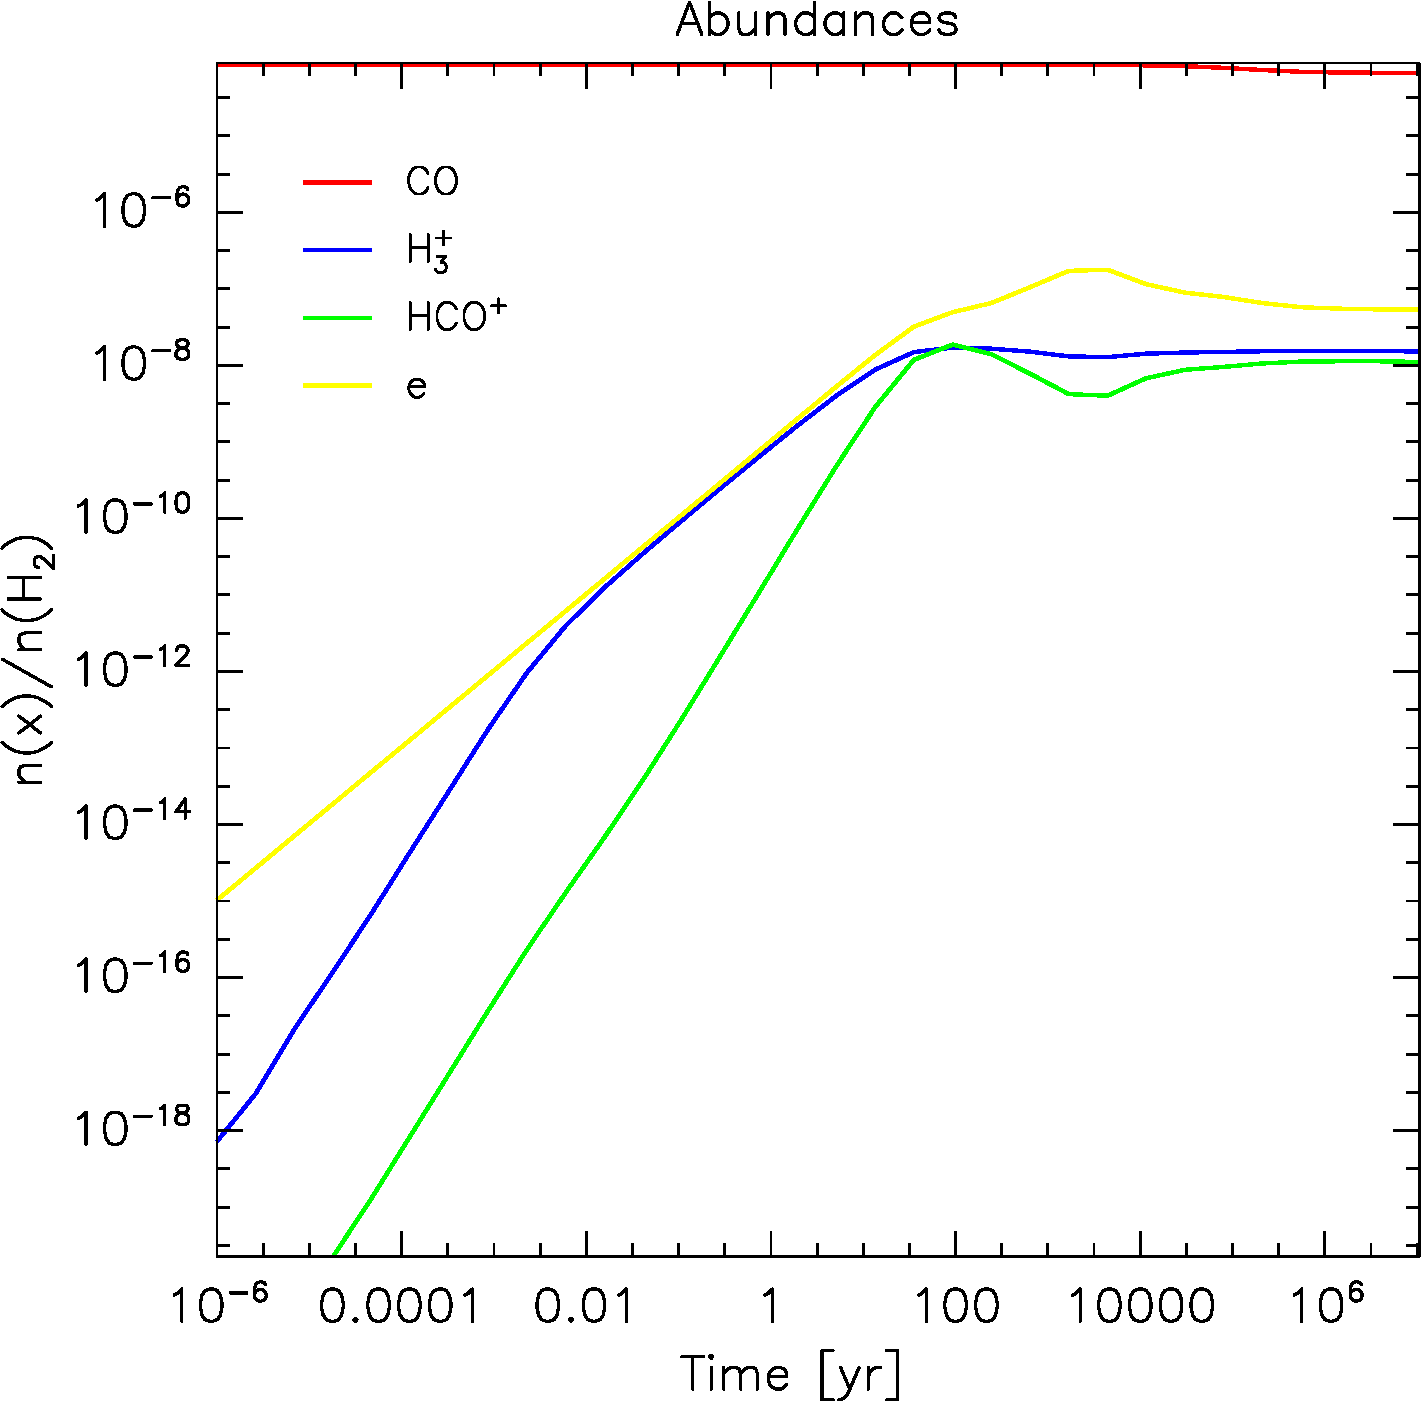
\includegraphics[width=10cm]{examples/abundances.pdf}
  \end{center}
  \caption{Abundances as a function of time for the example problem.}
  \label{fig:example-abundances}
\end{figure}

\noindent
This command produces the plot shown on
Fig.~\ref{fig:example-abundances}.

\section{Input file}
\label{sec:input-file}

This chapter describes the format of the input file used by Astrochem
(\verb=.ini= file). This file has several sections that are described
in the following.

\subsection{Files}
\label{sec:files}

This section of the file starts with the \verb=[file]= keyword, and
specifies which file Astrochem should use for the source description
(\verb=.mdl= file) and chemical network (\verb=.chm= file). The
parameters allowed in this section are:

\begin{itemize}

\item \verb=source=: The name of the file describing the source.

\item \verb=network=: The name of the chemical network file. This can
  be either a user written network (in the current directory), or one
  of the network provided with Astrochem.

\end{itemize}

\subsection{Physical parameters}
\label{sec:physical-parameters}

This section of the file starts with the \verb=[phys]= and specifies
the physical parameters of the problem. These parameters are:

\begin{itemize}

\item \verb=chi=: The external radiation field, expressed in Habing
  units. This corresponds to $\chi$ in Eq.~(\ref{eq:photo-ionization})
  and Eq.~(\ref{eq:photo-desorption}).

\item \verb=cosmic=: The cosmic ray ionization rate of molecular
  hydrogen expressed in s$^{-1}$. The default value is $1.3 \times
  10^{-17}$. This corresponds to $\zeta$ in
  Eq.~(\ref{eq:cosmic-ray-ionization}).

\item \verb=grain_size=: The grain radius in microns. The default
  value is 0.1. This corresponds to $r_{d}$ in
  Eq.~(\ref{eq:depletion}).

\end{itemize}

\subsection{Solver parameters}
\label{sec:solver-parameters}

This section of the file starts with the \verb=[solver]= and specifies
the parameters needed by the ODE solver. These parameters are:

\begin{itemize}

\item \verb=ti=: The initial time for the computation, expressed in
  years. The default value is $10^{-7}$.

\item \verb=tf=: The final time for the computation, expressed in
  years. The default value is $10^{7}$.

\item \verb=abs_err=: The solver absolute error on the computed
  abundances. The default value is $10^{-15}$.

\item \verb=rel_err=: The solver relative error on the computed
  abundances. The default value is $10^{-6}$.

\end{itemize}

\subsection{Initial abundances}
\label{sec:initial-abundances}

This section specifies the initial abundances in the computation. Each
line should contain a specie name followed by a equal sign and the
initial abundance with respect to H nuclei. Species abundances that
are not specified here are assumed to be zero.

\subsection{Output}
\label{sec:output}

This section specifies what output file Astrochem should create at the
end of the computation. These parameters are:

\begin{itemize}

\item \verb=output=: The name of the species for which Astrochem
  should create an output file containing the abundance as a function
  of time and position. Species names must be separated by a
  comma. File names are formed with the species name, possibly
  followed by a suffix (see below) and the \verb=.abun= file
  extensition.

\item \verb=suffix=: A suffix to append to the name of the specie,
  before the file extension (\verb=.abun= or \verb=.reac=). This is
  useful when you want to run astrochem for a number of different
  input files located in the same directory; this way the results of a
  given simulation won't be overwritten by results of an other one. A
  leading underscore will be added to this suffix.

\item \verb=time_steps=: The number of time steps in output files. The
  default value is 32. If plots of abundances v.s. time appear too
  ``boxy'', you may increase this number. Note that this only affect
  the number of time steps in the output files. The internal time step
  size is set by the ODE solver in order to reach the specified
  absolute and relative errors on the abundances.

\item \verb=trace_routes=: This parameter is used to toggle the
  computation of the major formation and destruction routes of the
  species given in @code{output}. If this parameter is set to 1,
  Astrochem will create a file that contain the formation/destruction
  rate and reaction number of the 10 most important
  formation/destruction reaction for each specie, as a function of
  time position (i.e. shell). As for abundance files, file names for
  formation and destruction routes are formed with the species name,
  possibly followed by a suffix (see below) but with the \verb=.reac=
  file extensition.

\end{itemize}

\section{Chemical networks}
\label{sec:chemical-networks}

Astrochem comes with several chemical networks files. You can also write
your own networks. This chapter describes the networks files provided
with Astrochem, as well as the network file format and reaction scheme
used by Astrochem.

\subsection{Networks provided with Astrochem}
\label{sec:netw-prov-with}

Several networks are distributed with Astrochem.  These networks can
be found in the network directory of the source distribution.

\begin{itemize}

\item \verb=osu2007.chm=: This network file contains the reactions and
  rates from the Ohio State University astrochemistry database, that
  is maintain by Eric Herbst. In correspond to the January 2007
  version of the database. This network contains 4429 reactions and
  452 species.

\item \verb=osu2005.chm=: This network corresponds to the 2005 version
  of the Ohio State University astrochemistry database.

\item \verb=osu2003.chm=: This network corresponds to the 2003 version
  of the Ohio State University astrochemistry database.

\item \verb=udfa2006.chm=: This networks contains the reactions and
  rate from the UMIST Database for Astrochemistry (UDFA) 2006, that is
  maintained Tom Millar and collaborators. This file correspond to the
  non-dipole version, that is it does not includes the enhancement of
  ion-neutral rates for reactions in which the neutral has a large,
  permanent dipole moment.

\item \verb=udfa2006_dipole.chm=: This network correspond to the
  dipole enhanced version of the UDFA 2006 database. It should be
  preferred to the non-dipole version for low temperaratures (a few
  tens Kelvins).  @end itemize

\end{itemize}

\subsection{Network file format}

This section describes the file format for Astrochem network files
(\verb=.chm=). Here is an example of a (incomplete) network file:

\begin{verbatim}
# A few reactions extracted from osu2008.chm
H2     + cosmic-ray  -> H2(+)  + e(-)        9.30e-01  0.00e+00  0.00e+00  1   39
H3(+)  + CO          -> HCO(+) + H2          1.61e-09  0.00e+00  0.00e+00  2 1756
H3(+)  + e(-)        -> H      + H      + H  4.36e-08 -5.20e-01  0.00e+00  9 3746
CO     + uv-photon   -> C      + O           3.10e-11  0.00e+00  2.54e+00 13 4297
(...)
\end{verbatim}

Lines that starts with the \verb=#= character are comments.

Each reactant and each products are separated by a \verb=+= sign
preceded and followed by one or more white space or tab. Up to three
reactants can be specified. Ions charges must be put between
paranthesis. Note that \verb=cosmic-ray=, \verb=uv-photon= and
\verb=photon= are not actual reactant or products, but just make the
reading of the network easier. They are ignored by Astrochem.

Reactants and products are separated by the \verb=->= characters. Up
to four products can be specified.

The five numbers following the products are the rate constants
\verb=\alpha=, \verb=\beta=, and \verb=\gamma=, the reaction type, and
the reaction number. The reaction types are given in
Table~\label{tab:react-type-numb}. The physical meaning of the rate
constants depend on the type of the reaction; the correspondance
between these constants and that used
Eq. (\ref{eq:grain-attach-neutralization}) to
(\ref{eq:photo-desorption}) is given in
Table~\label{tab:rate-const-meaning}.

\begin[h]{table}
  \begin{center}
    \caption{Reaction type numbers}
    \begin{tabular}{ll}
      \hline
      \hline
      Type number & Reaction type\\
      \hline
      0  & Gas-grain interaction, Electron-grain recombination\\
      1  & Cosmic-ray ionization or cosmic-ray induced photo-reactions\\
      2  & Ion-molecule reactions, Charge exchange reactions\\
      3  & Negative ion - neutral species reactions\\
      4  & Radiative association\\
      5  & Associative ejection\\
      6  & Neutral + Neutral $\rightarrow$ ion + electron\\
      7  & Neutral-Neutral chemical reactions\\
      8  & Neutral-Neutral radiative association\\
      9  & Dissociative recombination\\
      10 & Radiative recombination\\
      11 & Positive ion - Negative ion recombination\\
      12 & Electron attachment\\
      13 & Photo-ionization, Photo-dissociation\\
      20 & Freeze-out on grains\\
      21 & Thermal desorption\\
      22 & Cosmic-ray induced desorption\\
      23 & Photo-desorption\\
      \hline
    \end{tabular}
    \label{tab:react-type-numb}
  \end{center}
\end{table}

\begin[h]{table}
  \begin{center}
    \caption{Physical meaning of the rate constants used in chemical
      networks}
    \begin{tabular}{lcccc}
      \hline
      \hline
      Type number & Eq.\footnotemark[1] & \multicolumn{3}{c}{Rate constants\footnotemark[2]}\\
      \cline{3-5}
      & & $a$ & $b$ & $c$\\
      \hline
      0     & (\ref{eq:grain-attach-neutralization}) & $\alpha$ & $\beta$\\
      1     & (\ref{eq:cosmic-ray-ionization}) & $\alpha$ & - & -\\
      2-12  & (\ref{eq:arrhenius}) & $\alpha$ & $\beta$ & $\gamma$\\
      13    & (\ref{eq:photo-ionization}) & $\alpha$ & - & -\\
      20    & (\ref{eq:freeze-out}) & $S$ & $m/m_\mathrm{H}$ & -\\
      21    & (\ref{eq:thermal-desorption}) & - & $m/m_\mathrm{H}$ & $E_{b}$\\
      22    & (\ref{eq:cosmic-ray-desorption}) & - & $m/m_\mathrm{H}$ & $E_{b}$\\
      23    & (\ref{eq:photo-desorption}) & $Y$ & - & -\\
      \hline
    \end{tabular}
    \label{tab:rate-const-meaning}
    \footnotetext[1]{Equation used in the code to compute the rate}
    \footnotetext[2]{Rate constants used in the chemical network file}
  \end{center}
\end{table}

\subsection{Convert networks to Astrochem format}

Astrochem comes with a tool called \verb=chmconvert= to convert network
files to \verb=.chm= files. This tool support formats of the UMIST and
OSU database. The type of file is determined from the file extension,
which should be \verb=.udfa= for UMIST database files, and \verb=.osu=
for Ohio State University database files. Networks can be converted as
follows:

\begin{verbatim}
% chmconvert -o osu2007.chm osu2007.osu
\end{verbatim}

The \verb=-o= option is used to select the name of the output file. If
not specified, the network is copied to the standard output.

\section{Source model}
\label{sec:source-model}

\section{Plotting abundances}
\label{sec:plotting-abundances-1}

\section{Identifying formation and destruction routes}
\label{sec:ident-form-destr}

\bibliography{astrochem.bib}
\bibliographystyle{apj}

\newpage
\appendix

\section{List of contributing authors}

\section{Acknowledging Astrochem developers in your publications}

\end{document}
